\documentclass{article}
\usepackage[utf8]{inputenc}
\usepackage{graphicx} % Para incluir imágenes

\title{Reporte de Profiling de Código}
\author{Tu Nombre}
\date{\today}

\begin{document}
\maketitle

\section{Introducción}
Este reporte presenta el análisis de profiling del código para la probabilidad crítica $p_c \approx 0.59271$ y $L=128$.

\section{Metodología de Profiling}
Se utilizó la herramienta X para generar un flat profile del código. Los resultados se encuentran en profiling-report.txt.

\section{Resultados del Profiling}
A continuación se muestra un ejemplo de los resultados del profiling:CVCCCCCCCCCCCCCCCCCCCCCCCCCCCCCCCCCXXXXXXXXXXXXXXXXX
CDSCCXZCXCXCXsdcxcxcxcxcxcxcxcxcxcxcxxxxxxxxxxxxxxxxxxxxxxxxxxxxxxxxxxxxxxxxxxxxxxxxxxxxxxxxxxxxxxxxxxxxxxxxxxxxxxx
\begin{figure}[h!]
    \centering
    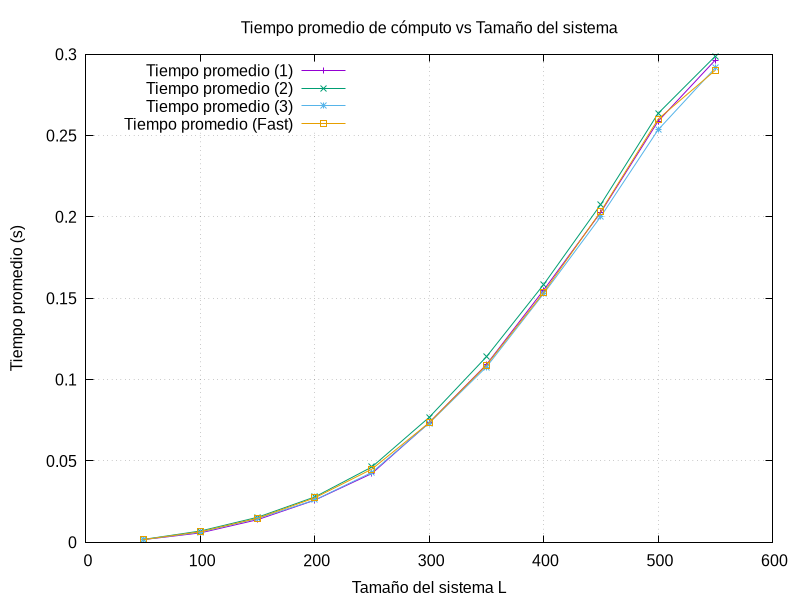
\includegraphics[width=0.7\textwidth]{tiempo_vs_L.png} % Asume que figura_profiling_ejemplo.png está en el mismo directorio o especifica la ruta
    \caption{Grafica del tiempo de computo (CPU) en funcion del tamaño del sistema L.}
    \label{fig:grafica}
\end{figure}

\section{Análisis y Optimizaciones}
El análisis del profile reveló que la función consume el 70\% del tiempo total de ejecución. Se implementó una optimización basada en cacheing que redujo su tiempo de ejecución en un 30\%.

\section{Conclusiones}
Las optimizaciones realizadas mejoraron significativamente el rendimiento del programa.

\end{document}